\chapter{文献综述}

为了更深入地研究上述问题,我们首先要明确安全库存、在途库存等概念的准确定义和计算方法,然后了解多阶段生产的特点以及用于研究多阶段生产的现有数学模型。






\section{安全库存和安全时间}

Fetter和Dalleck(1961) \cite{fetter_decision_1961} 认为安全库存是为了满足一定服务水平而保留的库存。作者根据日销售量和补货周期等因素,提出了计算一定服务水平下的安全库存的方法。

Lambrecht等人(1984) \cite{lambrecht_protective_1984} 在研究物料需求计划系统(MRP)时指出,安全库存是为了对抗需求预测、生产批量、生产运输提前期等因素中存在的不确定性。作者根据供应链中的级库存模型,将多阶段生产计划建模成动态规划问题和马尔科夫决策问题,改进了Clark和Scarf(1962) \cite{clark_approximate_1962} 的启发式算法,并指出了启发式算法的上下界和获得最优解条件。

Baker等人(1986) \cite{baker_effect_1986} 研究了多阶段生产线中,提高零部件通用性对安全库存的影响。作者结合风险分担思想在供应链等领域中的应用,用数学模型证明,在给定最低服务水平的情况下,引入通用件能够降低两阶段、两产品生产线的安全库存,并总结了引入通用件产生的影响:
所有零件的安全库存总数降低;
通用件的安全库存低于它所替代的两种零件安全库存之和;
没有被通用件替代的其他零件安全库存增加。

Eppen和Martin(1988) \cite{eppen_determining_1988} 总结了各种情况下安全库存的计算方式。
当需求和提前期分布已知时,令$W$代表提前期内需求,$X$代表单位时间需求,$Y$代表提前期长度,$R$代表补货点。则有以下公式。
\begin{align}
\mu_W &= \mu_X \mu_Y \\
\sigma_W^2 &= \sigma_X^2 \mu_Y + \sigma_Y^2\mu_X^2 \\
R &= \mu_W + Z_\delta \sigma_W
\end{align}
当需求和提前期分布未知时,需要视情况建立合适的模型估算它们的分布。

Molinder(1997) \cite{molinder_joint_1997} 认为生产中的不确定性主要来自需求、制造、运输等环节,并进一步指出制造环节的不确定性是由产能负载、机器故障、排队效应、返工等多种因素引起的。作者认为这些不确定性对多阶段生产的影响尤其显著,因为某一工序的延迟可能导致物料清单(BOM)上所有更高级别的物料都受到影响。作者通过模拟退火优化了多种参数情形下的订货批量、安全库存和提前期,并比较了每种情形下用安全库存或安全时间作为对抗风险准则的效果。实验结果表明:
\begin{enumerate}
\item
需求不确定性高、提前期不确定性低时,宜采用安全库存作为优化准则;需求和提前期不确定性都高时,宜采用安全时间作为准则。
\item
产品结构(或BOM)基本不影响采用哪种准则的抉择。
\item
当缺货成本与库存成本之比较低时,安全库存准则比其他准则都好。
\item
当上述比值较高时,准则的抉择往往取决于需求不确定性。需求不确定性低,宜采用安全库存;反则宜采用安全时间。
\end{enumerate}

Chopra等人(2004) \cite{chopra_effect_2004} 认为降低供应商的供货提前期和降低供货提前期的不确定性是两种降低安全库存的有效方法。一般认为,在正态模型下,降低供货提前期的不确定性比降低供货提前期更为有效,尤其是在供货提前期不确定性较大的情况下。本文作者以Eppen和Martin(1988) \cite{eppen_determining_1988} 的工作为基础,证明了该结论不是完全正确的,而是存在一个不小于50\%的服务水平临界点,当服务水平低于这个临界点时,降低提前期的不确定性反而会使安全库存增大。若模型是正态的,则这个临界点为50\%;若不是正态的,临界点一般在50\%到70\%,正好是一般企业的服务水平范围。因此企业如果希望降低安全库存,必须谨慎检查自己的服务水平和提前期分布模型,盲目降低提前期的不确定性反而可能增大安全库存。文章的最后,作者还提出了通过累积分布函数(CDF)估算临界点的方法。

Fang等人(2013) \cite{fang_decision_2013} 考虑需求不确定性、提前期、提前期不确定性的边际价值,建立了能同时处理需求和供应两边不确定性的模型,并且不依赖于最优库存策略。相反,非最优的库存策略下,从这几个方面获得的边际价值更大。因此,即使面临糟糕的库存管理策略,管理人员也能够根据此模型很快找出最有效率的改进方向。







\section{多阶段生产和在途库存}

Gershwin(1994) \cite{gershwin_manufacturing_1994} 研究了如图 \ref{fig:transfer_line} 所示的单产品多阶段生产线。其中$M_i$代表机器,$B_i$代表缓存。

\begin{figure}[htbp]
\centering
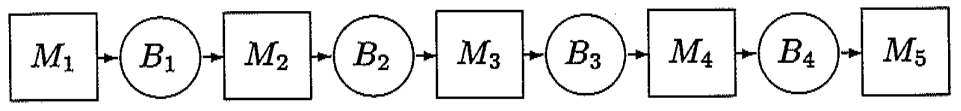
\includegraphics[width=12cm]{transfer_line.png}
\caption{单产品多阶段生产}
\label{fig:transfer_line}
\end{figure}

多阶段生产中的重要制约因素是机器故障。机器故障有两种模式:基于时间的故障模式和基于运作的故障模式。两种模式都是随机的。基于时间的故障模式下,机器故障的发生取决于使用的时间长短,比如材料的强度失效;基于运作的故障模式下,机器故障的发生取决于使用次数或产量,比如刀具失效。

机器即使没有出故障,也不一定能运转,因为还受到上下游库存的限制。如果上游库存不足,导致下游机器停工,我们称下游机器为缺料状态;如果下游库存已满,导致上游机器停工,我们称上游机器为阻塞状态。

缓存区的库存被称为在途库存。在多阶段生产中,在途库存往往是必不可少的,因为它能减少机器故障带来的损失。当一台机器出现故障时,上游的机器可以继续运转,生产的产品进入在途库存;下游机器也能依靠故障机器的在途库存提供原料继续运转。但在途库存也会带来一些问题,Gershwin在书中总结了在途库存的主要缺点:
\begin{enumerate}
\item
在途库存是消耗资金制造出来的,占用了资金却不产生任何效益。
\item
根据Little's Law \cite{little_proof_1961} ,在途库存对提前期有影响。在途库存越多,提前期越长。提前期过长可能导致顾客不满,同时也使得生产中的故障更难以被观察到。在观察到故障之前,故障机器可能已经制造了很多残次品。
\item
零部件在库存期间可能遭受破损、偷窃等损失。库存量越大、时间越长,遭受的损失越大。
\item
储存用的场地和设备会消耗空间和资金。
\end{enumerate}

Gershwin还用马尔科夫模型分析了多阶段生产线在缓存容量上限$N=0$和$N=\infty$的极端情形下的表现,得出了两个重要的结论:
\begin{enumerate}
\item
在$N=0$的情况下,多阶段生产线的运作时间与总时间之比总是随机器数目增加而减小,并且收敛于0。也就是说,如果没有在途库存,当产品需要的生产阶段很多时,生产线的效率将趋近于0。
\item
在$N=\infty$的情况下,多阶段生产线的产能总是取决于最慢的一台机器。也就是说,总体产能只有在瓶颈阶段可能得到优化。
\end{enumerate}

Gershwin指出,用马尔科夫模型研究多阶段生产还存在一些难点。最突出的难点就是状态空间过大。每个机器有2种状态,每个缓存有$N+1$种状态,马尔科夫模型的状态空间就是它们的乘积,即
\[
M = 2^k \prod_{i=0}^{k-1}(N_i+1)
\]
随着阶段数目的增加,状态空间$M$很快就变得非常庞大。

Goyal(1978) \cite{goyal_economic_1978} 考虑需求分布均匀、不允许缺货的多阶段生产,建立了以减少总成本为优化准则的数学模型,用于分析最优的生产批量以及各阶段之间最优的运输批量。

Kimura和Terada(1981)\cite{kimura_design_1981} 分析了多阶段拉动式生产的需求和库存波动是如何逐级传递的,证明了拉动式生产系统比推动式生产系统更能适应需求的波动,并能够防止下游的生产和库存波动向上游逐级扩大。Kimura和Terada所定义的拉动式生产系统需要满足以下运行方式:建立标准的再订货点和订货批量大小;随时了解库存水平和延期订单;连续检查库存水平,一旦某些零部件数量低于再订货点,就立即向上游订货。拉动式生产系统中使用看板来维持运作,流程如图 \ref{fig:pull_system} 所示。

\begin{figure}[htbp]
\centering
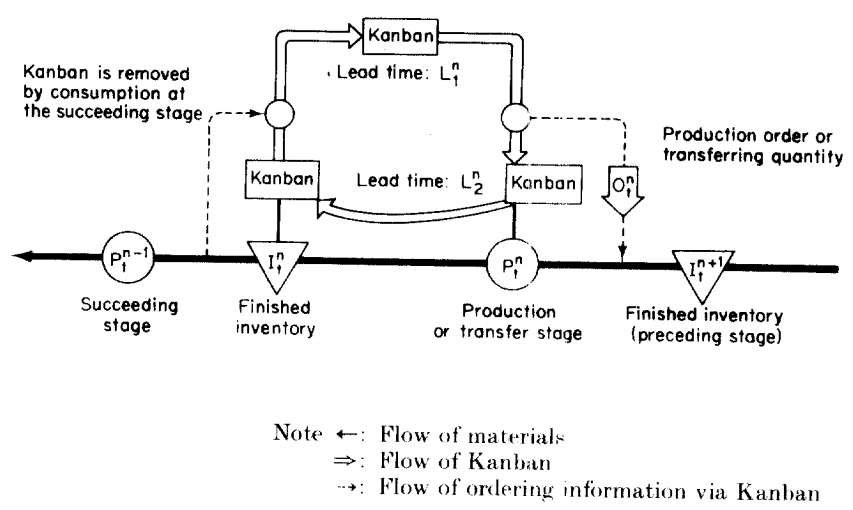
\includegraphics[width=12cm,angle=1,origin=c]{pull_system.png}
\caption{拉动式生产系统流程图}
\label{fig:pull_system}
\end{figure}

研究中使用的推动式生产系统是Tabe等人(1980) \cite{tabe_analysis_1980} 建立的模型,如图 \ref{fig:push_system} 所示。

\begin{figure}[htbp]
\centering
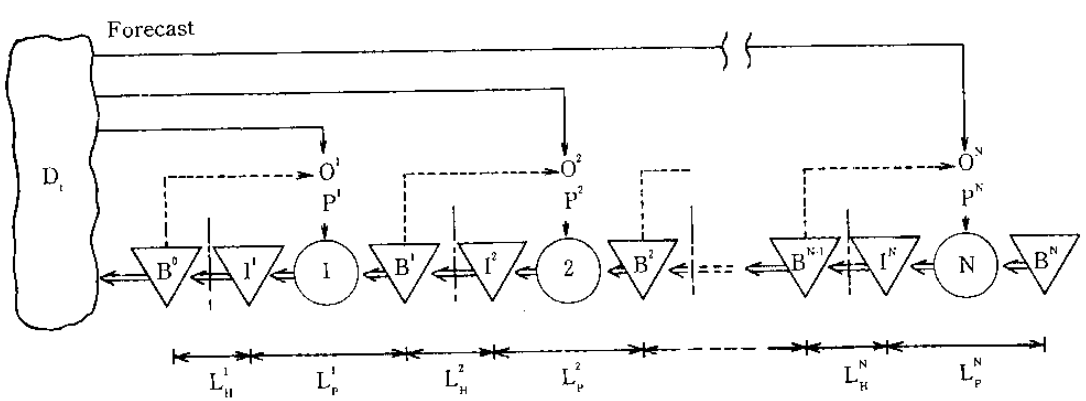
\includegraphics[width=12cm,angle=-1,origin=c]{push_system.png}
\caption{推动式生产系统流程图}
\label{fig:push_system}
\end{figure}

通过数学模型分析和仿真模型实验,Kimura和Terada得到如下结论:
\begin{enumerate}
\item
拉动式生产系统中,单位订货量的大小非常重要。在单位订货量与产量水平相比很小的情况下,拉动式生产中的下游生产波动不会在向上游传递的过程中放大。
\item
推动式生产系统中,生产和库存波动的放大率取决于预测误差。以波动放大率为准则时,推动式系统和拉动式系统之间的抉择取决于预测误差的大小。
\item
拉动式生产系统中另一个影响波动放大率的参数是从看板离开容器到该阶段完成生产的时间差。这个时间差越长,波动放大率越高。
\end{enumerate}

Conway等人(1988) \cite{conway_role_1988} 反对一味追求降低在途库存的做法,全面总结了在途库存在多阶段生产中的意义和作用,并分析各种情况下如何真正改善多阶段生产的绩效。该研究中有以下一些重要的结论:
靠前的几个阶段对整条生产线的产能影响最大,长生产线的绩效比短生产线差得不多;
添加缓存对绩效的提升较大,但增加缓存容量的效果不显著;
在生产线靠中间的位置添加缓存,效果比靠两端的位置好得多;
在未平衡的生产线中添加buffer效果不显著。








\section{风险分担}

已读17篇risk pooling相关文献,待补充文献综述。











\section{延迟差异化}

已读10篇postponement相关文献,待补充文献综述。